\documentclass[aps,prl,10pt,twocolumn,floatfix]{revtex4-2}
\usepackage{graphicx}
\usepackage{dcolumn}
\newcolumntype{d}{D{.}{.}{-1}}
\usepackage{url}
\usepackage{physics}

\bibliographystyle{apsrev4-2}


\begin{document}

%\begin{abstract}
%\end{abstract}


\title{Measuring the Universal Gravitation Constant with the Cavendish Balance}
\author{C. T. Rochelle}
\email{ctr233@msstate.edu}
\author{K. J. Grimes}
\date{\today}
\affiliation{Department of Physics and Astronomy\\Mississippi State University\\Mississippi State, MS 39762-5167}
\date{\today}

\maketitle

\section{Introduction}\label{Intro}
% Lead Up to Creation
One of the most important constants in all domains of physics is the Universal Gravitation constant. 
It is used to determine the orbits of planets and galaxies as well as interactions between the smallest known particles.
Since every single object in the universe is subject to this fundamental force, its precise calculation is very important.
This has led to many physicists and scientists trying to obtain smaller uncertainties and higher precision over the decades since its formulation. 

The first measurement for the Universal Gravitation constant was in 1789 by Lord Henry Cavendish \cite{class}, whose name the instrument used in this experiment was named after. 
He used the design and methods laid out by the astronomer John Michell, who passed a few years prior before he could complete the experiment himself \cite{birtanica}. 
While this was the first experimental measure of the gravitational constant, it was not intended to be. 
Cavendish and Michell intended it to measure the density of the Earth, which was later extrapolated to determine the measure of the constant \cite{britanica}.
This experiment was impactful not only because it measured the average density of the Earth accurately, but also because it showed that all atoms in the universe were subject to the laws of gravity, all with the same constant. 

\section{Theory}\label{Theory}
% Explanation of Inner Workings
In the Cavendish experiment, a torsion balance is used to measure the impact of the gravitation constant on the torque of the wire holding two smaller masses, being pulled toward two larger masses. 
The goal of this experiment is to convert the measure of torque in the system to arrive at our value. 
To do this, we must derive a formulation to take that torque and other known properties of the system to calculate the constant of gravitation. 

% Derivation of Formula 
We will start with the equation of torque: 
\begin{equation} \label{torque}
\tau = F \cross d
\end{equation}
where $\tau$ is the torque, $F$ is force, and $d$ is the distance from the center the force is being applied. 
Since there are two masses at the same distance away from center, the torque of the system is twice the regular formula.
The force we are trying to measure is that of the gravitational constant, which is $F_G=\frac{G M m}{r^2}$, where $r$ is the distance between the centers of the larger and smaller masses.
Making these changes to equation \ref{torque}, we get:
\begin{equation}\label{tauG}
\tau_G=2\frac{G M m}{r^2} d
\end{equation}
Another equation for $\tau_G$, which we will equate to \ref{tauG}, is the restoring torque from the string connecting the anchor point at the top of the device to the rotational element. 
It is given by: 
\begin{equation}
\tau_{res}=k\alpha
\end{equation}
where $k$ is the torsion constant of the string and $\alpha$ is the rotational acceleration. 

We now have the main equation to solve for $G$:
\begin{equation}
G=\frac{k\alpha r^2}{2M m d}
\end{equation}
It is easy to see how we would find $r$, $M$, $m$, and $d$, but $k$ and $\alpha$ require some some extra work.
We can measure both but looking at the oscillations of the rotational element while under the influence of the gravitational force of the large mass.

We know from classical mechanics that:
\begin{equation}
\tau_{res}=k\theta=I\ddot{\theta}
\end{equation}
We know that $\dot{\theta} = \omega$, so we can solve for k:
\begin{equation}
k=I\omega^2
\end{equation}.
Looking at the equation for the damped harmonic oscillator, we see we can find $\omega$ and $\alpha$:
\begin{equation}
\theta = Ae^{-\gamma t} \cos{(t\sqrt{\omega^2-\gamma^2}+\phi)}+\alpha
\end{equation}
where $A$ is the initial amplitude of oscillation, $\gamma$ is the dampening coefficient, $\phi$ is the offset angle, and $t$ is the time.
We obtain these values by fitting the data to a known function to determine $\omega$ and $\alpha$.

The last needed value that isn't measured directly is the inertia of the bar. 
This value is calculated by first calculating the inertia as if the bar had no cut-outs, then subtracting the inertias of the missing sections. 

Having done all of this, we will get an accurate answer for the gravitational constant:
\begin{equation}
G=\frac{I\omega^2\alpha r^2}{2M m d}
\end{equation}

\section{Experiment}
% What did you do?
This experiment begins by obtaining accurate measurements of the masses of all four masses and their diameters. 
Next, measure dimensions of the apparatus, namely: the distance between glass plates, thickness of the plates, and distances between the inner edges of the slots for the glass plates.
Lastly measure the length of the tungsten filament from the anchor point on the top of the apparatus to the connection of the rotational element. 
All of these values and their intermediary values used to calculate the moment of inertia of the bar are located in Figure \ref{measure}.

% Schematic
This section involves taking the data with the Cavendish Balance, pictured in Figure \ref{bal}.
To initialize and calibrate the system we needed to preform a few steps. 
The balance was placed on a slab on a tub of sand to reduce any external vibrations from outside the system and all masses were placed in their spots, making sure to place each smaller and larger masses simultaneously to avoid introducing unwanted vibrations.
One side plate was removed and the internal system (the internal ball and small masses) was balanced using the slider connected to the end of the wire suspending it, replacing the side plate when done.
The TEL-Atomic Voltage offset device was plugged into a nearby computer with the Cavendish data software installed. 
With the correct port selected (which needs to be determined each run), we set the recording frequency to $0.5 Hz$ and used the knob on the offset device to set the internal bar's resting value to approximately $0V$. 
With the initial value set, we slowly moved the external bar to the most extreme counter clockwise direction and started recording data.
We did this to introduce roughly the same energy into the system when we swing the bar in the full clockwise direction mid data collection. 
We recorded data in this position before swinging it to the extreme clockwise direction and back again. 
For the first, second, and third section, we waited to record at least 5 full oscillations of the internal bar before moving to the next section or stopping data collection. 
When transitioning between each data collection region, it was important swing the external bar in another direction only at the extrema of the oscillations of the internal bar. 

To determine the conversion between voltage recorded in the software to the angle the bar as moved, we recorded data using the Cavendish data software.
We removed the closest side plate and started recording data.
We slowly moved the internal bar until it touched the other side panel to measure the recorded voltage of the most extreme twist in one direction.
Once held steady to obtain that side's maximum, rotate the internal bar to the extreme with the other corner touching the side panel and hold it steady to record that side's max.
We recorded the angle the internal bar rotated in both steps to create a conversation factor. 

\section{Data Analysis}
% Explain the Results 

Figure \ref{dataOrigin} contains the plot and fits of each region of data collection in the Origin software. 

\begin{figure}
\centering
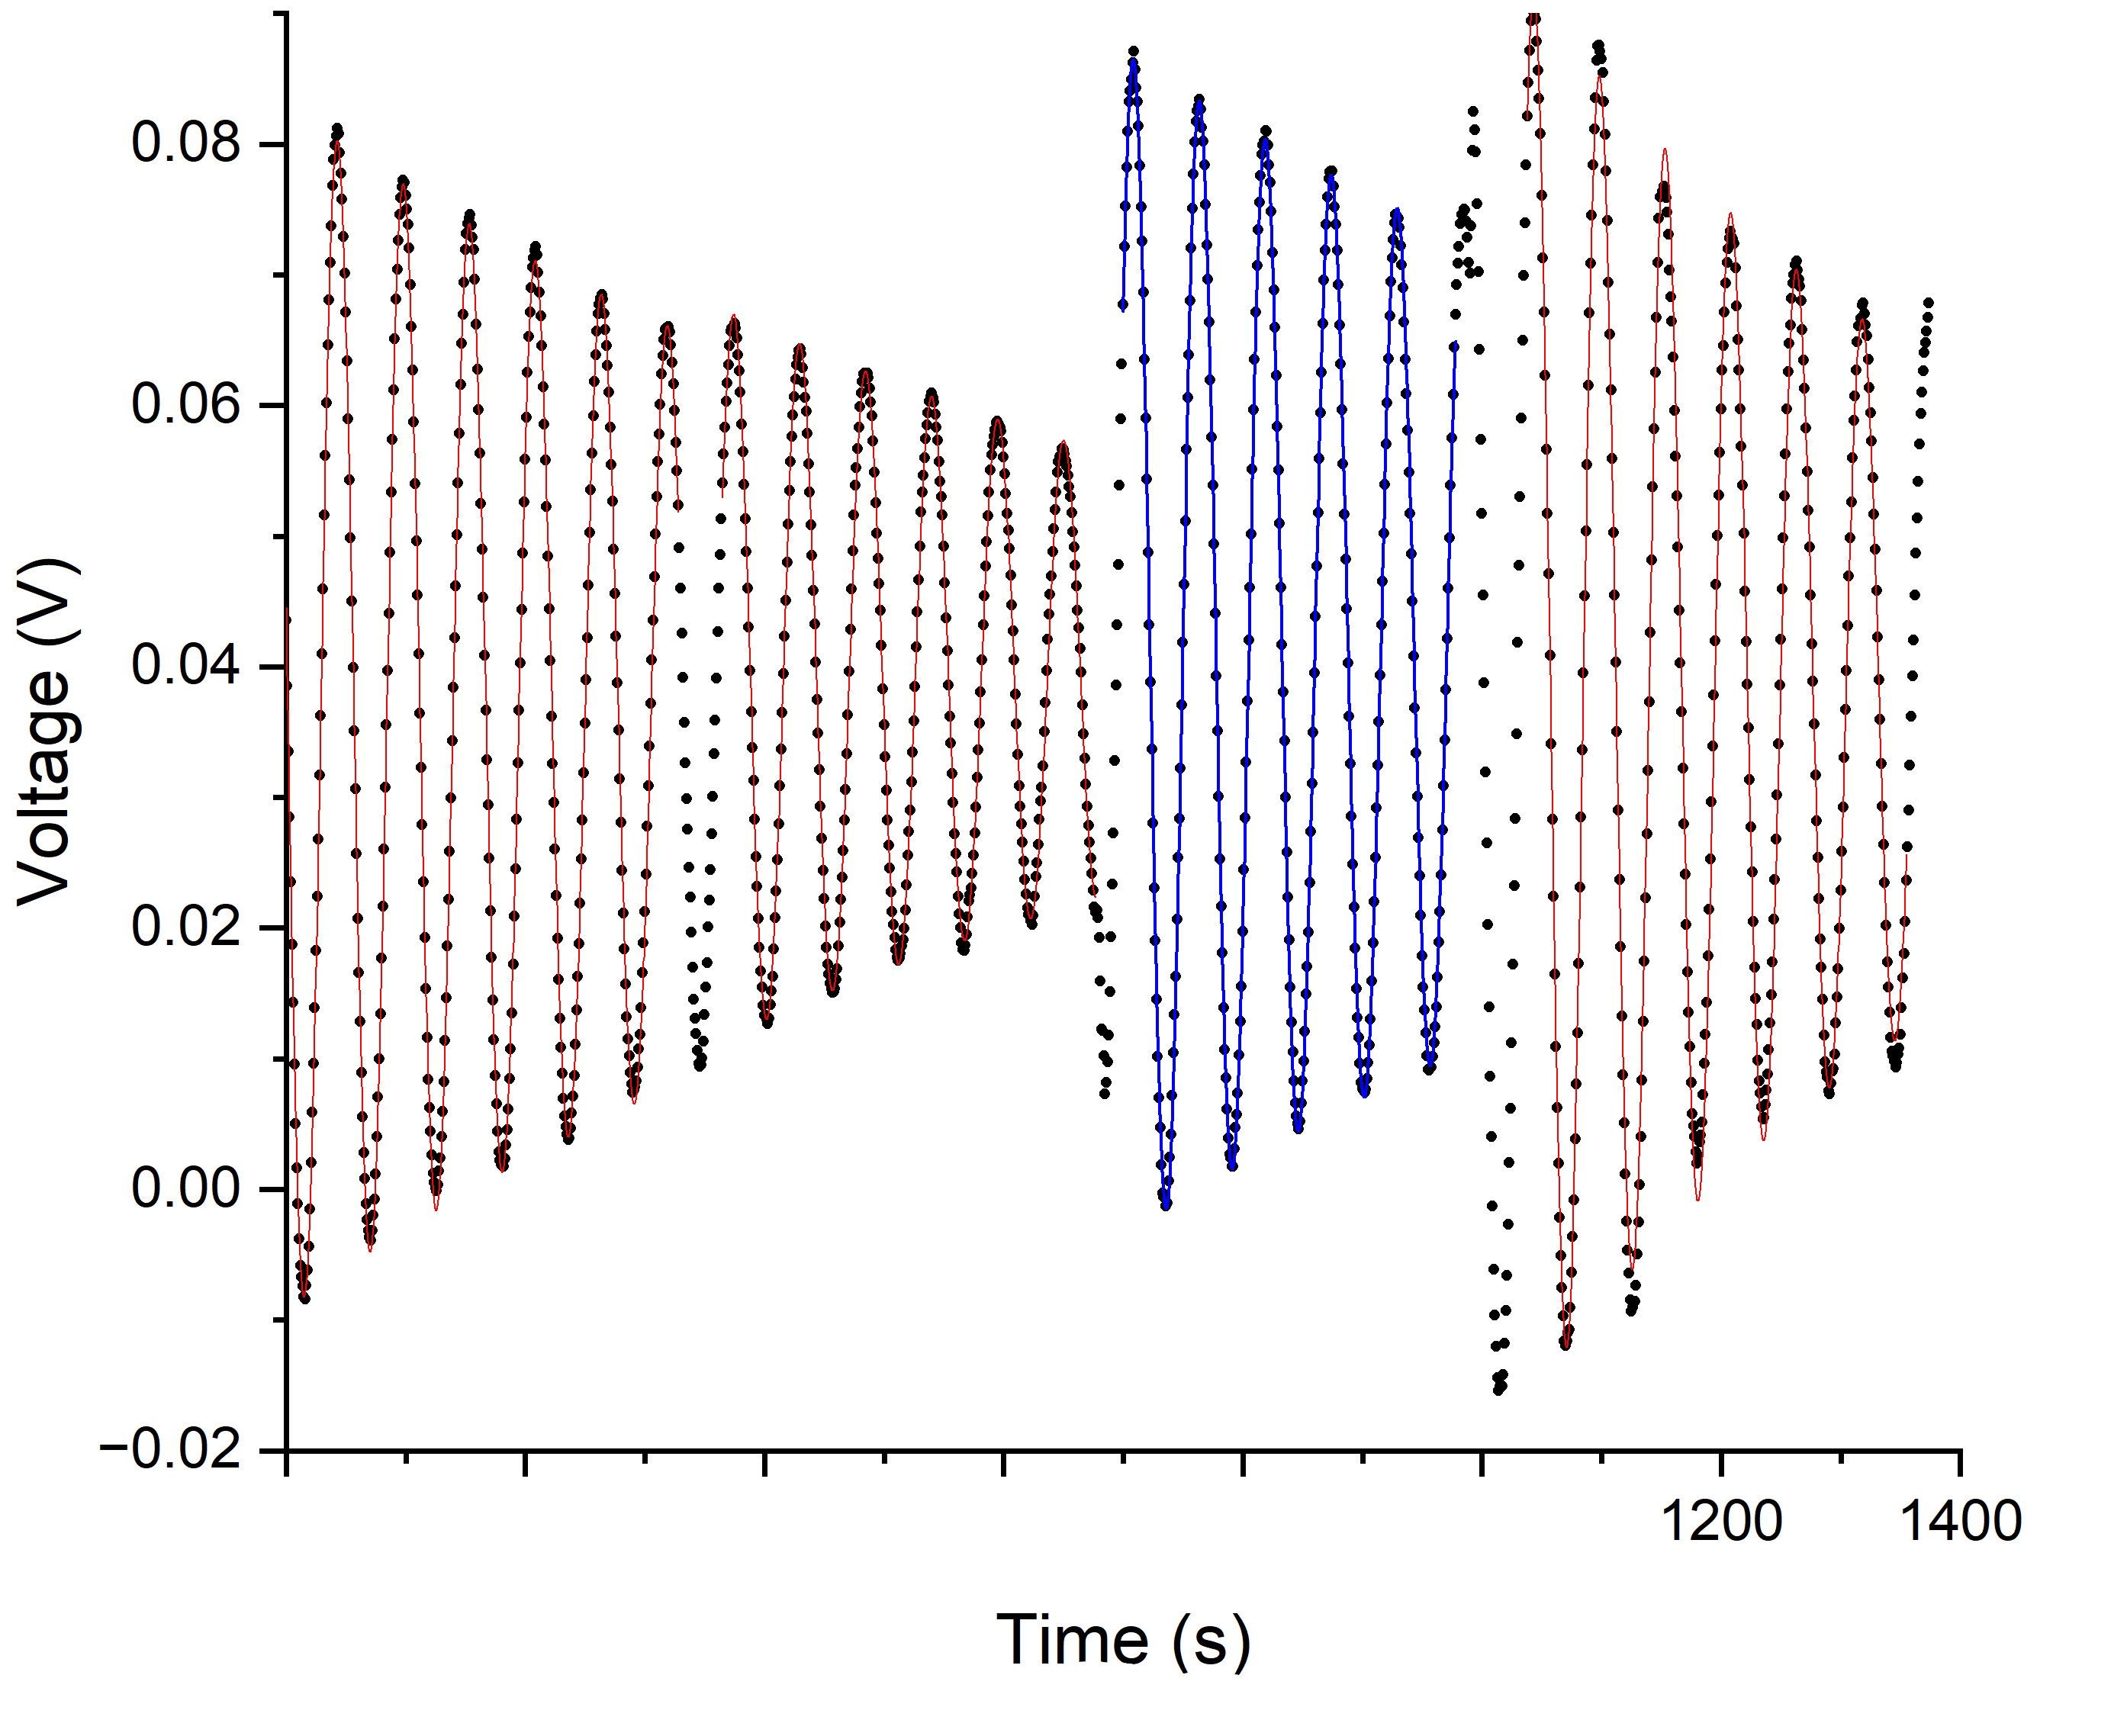
\includegraphics[width=20em]{dataOrigin.png}   
\label{dataOrigin}
\caption{A plot of the raw data and fits graphed in the Origin software. The first region, with the red fit, is the initial counter-clockwise position. The second region, with the blue fit, is the clockwise position. The last region, with the coral fit, is the final counter clockwise position.}
\end{figure}

Table \ref{measure} contains all of the constant values used to calculate the moment of the inertia of the bar, $I_D$.

\begin{figure}
\begin{tabular}{ |c c| } 
\hline
\multicolumn{2}{|c|}{Constants for $I_D$}\\
\hline
Parameter & Value \\
$M_1$ & 875.0(1) $g$ \\
$M_2$ & 884.0(1) $g$ \\
$m_1$ & 14.6328(1) $g$ \\
$m_2$ & 14.5880(1) $g$ \\
$d_{M1}$ & 54.07(1) $mm$\\
$d_{M2}$ & 54.78(1) $mm$\\
$d_{m1}$ & 13.54(1) $mm$\\
$d_{m2}$ & 13.50(1) $mm$\\
$t_{frontglass}$ & 2.78(1) $mm$\\
$t_{backglass}$ & 2.81(1) $mm$\\
$t_{rightofbox}$ & 38.20(1) $mm$\\
$t_{leftofbox}$ & 38.42(1) $mm$\\
$d_{separationofglass}$ & 28.70(3) $mm$\\
$d_{outeredgeofbox}$ & 2.01(1) $mm$\\
$l_{wirelength}$ & 61.20(5) $mm$\\
\hline
$V_{entirebeam}$ & 17.184(25) $cm^2$\\
$\rho$ & 0.4175(8) $cm^3$\\
$m_{leftslot}$ & 0.033 61(30) g\\
$m_{rightslot}$ & 0.026 93(21) g\\
$m_{innerslot}$ & 0.1044(6) g\\
$m_{circleslot}$ & 0.2959(17) g\\
$I_{entirebeam}$ & 148.24(34) g\\
$I_{innerslot}$ & 0.009 24(5) $gcm^2$\\
$I_{leftslot}$ & 1.8211(22) $gcm^2$\\
$I_{rightslot}$ & 1.4592(16) $gcm^2$\\
$I_{circleslots}$ & 26.29(15) $gcm^2$\\
$m_{leftmass}$ & 14.6328(1) $g$\\
$m_{rightmass}$ & 14.5880(1) $g$\\
$I_{beam}$ & 118.7(4) $gcm^2$\\
$_{Ileftmass}$ & 650.95(13) $gcm^2$\\
$I_{rightmass}$ & 648.95(13) $gcm^2$\\
\hline
$I_D$ & 1418.6(4) $gcm^2$\\
\hline
\end{tabular}
\label{measure}
\caption{A list of constants related to the calculation of the moment of inertia of the bar.}
\end{figure}

\begin{figure}
    \begin{tabular}{ |c c c c c c| } 
    \hline
Position& T (period)&b&A&theta&V (alpha)\\
\hline
Equilibrium &55.217(8)& 0.001430(17)& 0.04610(13)& 1.4045(28)& 0.036890(42)\\
CCW&55.199(32)& 0.001570(27)& 0.0495(6) &1.372(13)& 0.039430(35)\\
CW& 55.180(14) &0.001320(30)& 0.1143(25) &7.291(23) &0.04169 (6)\\
CCW&54.920(28) &0.00229(6)&0.584(31)&0.02(6) &0.03811 (11)\\
\hline
\end{tabular}
\label{final}
\caption{A list of constants related to the calculation of the moment of inertia of the bar.}
\end{figure}

\section{Conclusion}
% Conclusion 
The value for universal gravitation constant we found in this experiment was $G=7.06(52)\times 10^{-11} \frac{Nm^2}{kg^2}$, which is within $2\sigma$ of the accepted value, $G=6.67430(15)\times 10^{-11} \frac{Nm^2}{kg^2}$.
The issue with our final value is that the precision is low compared to the accepted value.
The uncertainty is so high because of a few reasons.
The spherical masses and bar are assumed to be perfect geometric shapes in the calculation of the moment of inertia of the bar;
however, the real masses and bar are not perfect and have imperfections (especially the spherical masses that have many dents).
The biggest introducer of uncertainty is the method of rotating the bar.
Ideally, the bar would be rotated to the far left and far right completely smoothly, with no jerking while introducing as little momentum from the swing as possible. 
This was not possible in practice was the bar was not well lubricated, forcing us to rotate the bar above some minimum speed to avoid the bar from seizing and making the bar jerk.
If given the chance to redo this experiment, we would lube the bar to allow us to slowly and smoothly rotate the bar around its pivot and use new masses that were more ideally spherical. 


%\begin{thebibliography}{9}
%\bibitem{light} \textit{The Speed of Light}, Las Cumbres Observatory. (May 4, 2022). \url{https://lco.global/spacebook/light/speed-light/#:~:text=Galileo\%20concluded\%20that\%20the\%20speed,one\%20person\%20to\%20the\%20other.}.
%\bibitem{engineer} C. McFadden, \textit{Physics in a Nutshell: A Brief History of the Speed of Light}, Interesting Engineering. (Apr 25, 2017). \url{https://interestingengineering.com/a-brief-history-of-the-speed-of-light}.
%\bibitem{NIST} \textit{speed of light in vacuum} (National Institute of Standards and Technology, May 4, 2022).
%\end{thebibliography}

\end{document}
